\RequirePackage{fix-cm}
\documentclass[10pt,journal,compsoc]{IEEEtran}
\usepackage{cite}
\usepackage{graphicx}
\usepackage{multirow}
\usepackage{hhline}
\usepackage{comment}
\usepackage[dvipsnames]{xcolor}
\usepackage[colorlinks=false, linkcolor=blue, citecolor=blue, bookmarks=true,pagebackref=false]{hyperref}
\usepackage{subcaption}
\usepackage{float}
\usepackage{caption}
\usepackage{fancybox}
\usepackage{array,booktabs}
\usepackage{marvosym} % For the \Letter command
%\usepackage{textcomp} % arrow
%\usepackage{tablefootnote} % footnote in table
\usepackage{balance}
\usepackage{ragged2e}
\usepackage{makecell}
\usepackage{bigstrut}
%\usepackage[title]{appendix}

\begin{document}
	\begin{appendices}
%=================== Model construction =================%
	This appendix will be available online~\cite{appendix}. We included it as supplementary material for the convenience of the anonymous reviewers.

      \section{Model construction}
      In this section, we elaborate on the details of our model construction process. Figure~\ref{fig:flowMC} shows an overview of our model construction process. The process can be broken down into following three steps:
	
	  \begin{figure}[b]
        \centering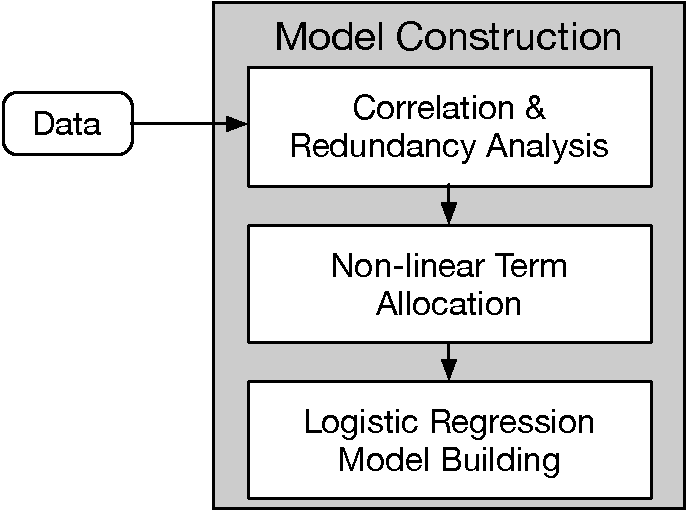
\includegraphics[width=.7\columnwidth]{pics/appendix/mondelconstruction}
        \caption{The overview our model construction process.}
        \label{fig:flowMC}
        \vspace{-0.2in}
      \end{figure}
	
	\begin{enumerate}
		\item \textbf{Correlation \& Redundancy Analysis:}  Similar to prior studies~\cite{gopi:2017,wang2017understanding,mcintosh2016empirical,kabinna2018examining}, we remove correlated and redundant factors to avoid multicollinearity.
      First, we use the Spearman rank correlation test to measure the correlation between factors and remove highly-correlated factors (using a cut-off value of 0.7 \cite{gopi:2017,wang2017understanding,mcintosh2016empirical,kabinna2018examining}). For each of the highly-correlated factors, we keep one factor in the model. Figure~\ref{FINAL_RQ3_hie} shows the results of our correlation analysis, and the factors that were eventually used in the models. Then we apply a redundancy analysis and remove redundant factors.
      Finally, we end up with three factors in the project bounty dimension, six factors in the issue report basic dimension, four factors in the issue report bounty dimension, and three factors in the backer experience dimension.
      Because factors which have a constant value do not contribute explanatory power to a logistic regression model, we remove factors which are constant within a project group when building the corresponding models. For example, we remove \textit{P\_B\_usage\_group} (i.e., bounty-usage frequency) for the first-timer models , the moderate models and the frequent models since \textit{P\_B\_usage\_group} is a constant value for these models. In addition, we remove all project bounty-related factors for the first-timer bounty-projects since for these projects the values of all project bounty-related factors are 0.

	
      \begin{figure}[t]
        \centering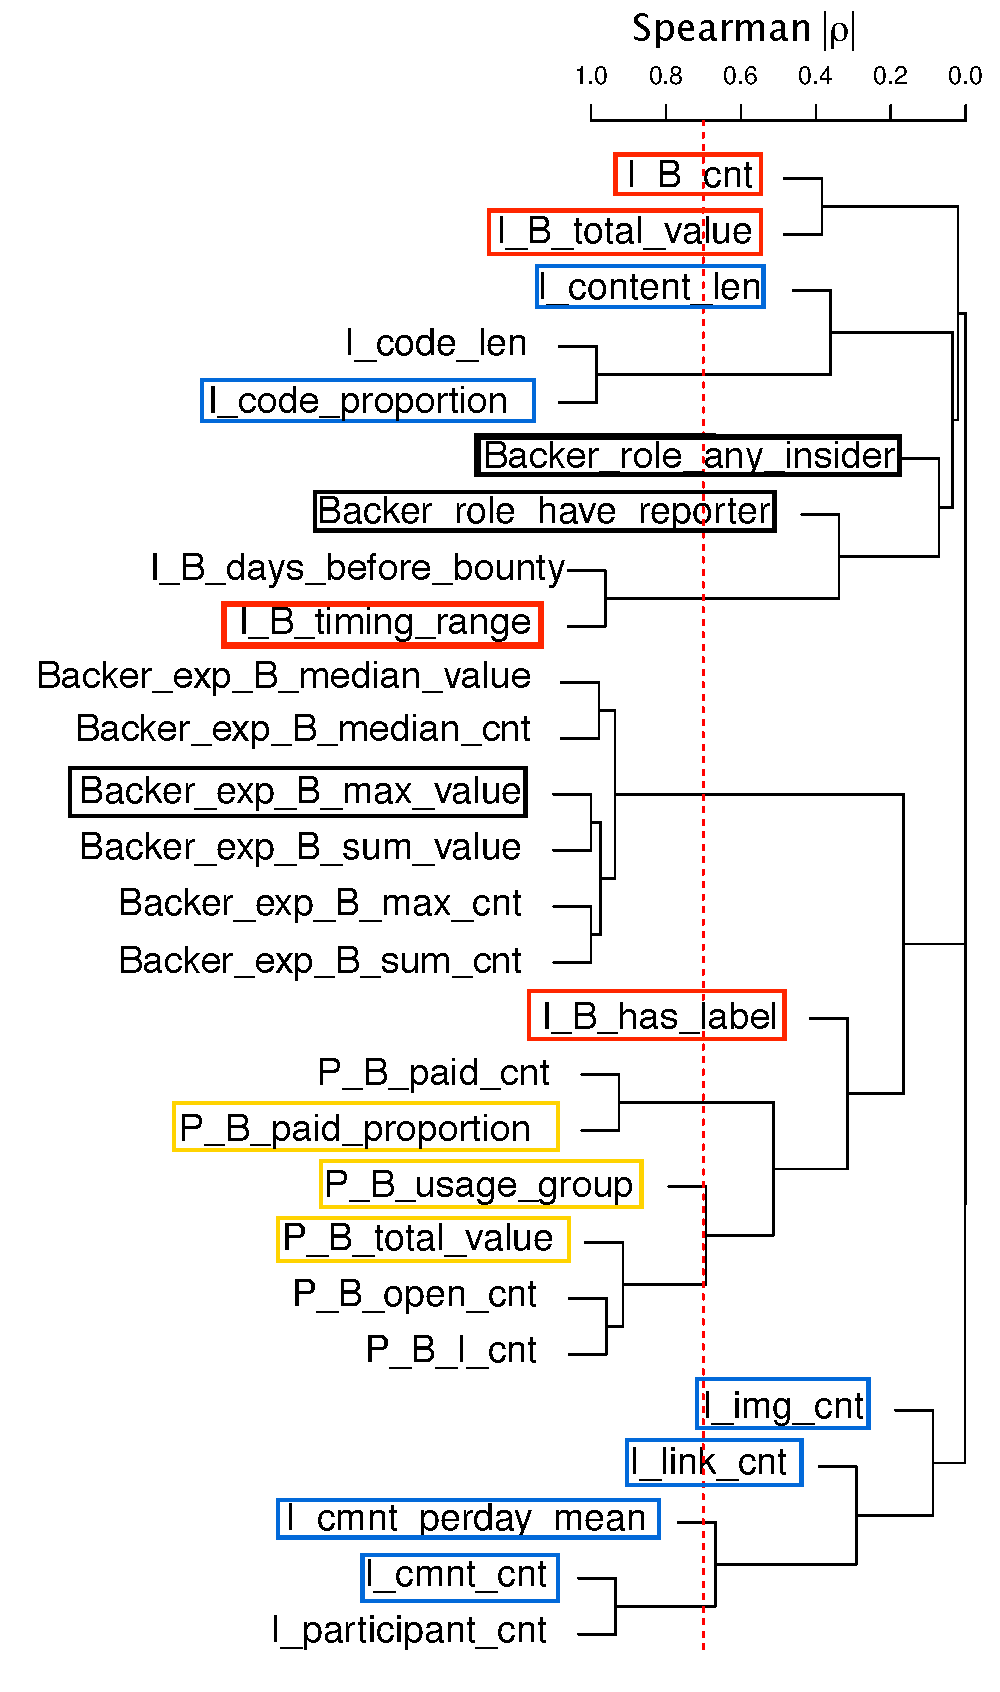
\includegraphics[width=\columnwidth ]{pics/rq3/rq3_hie}
        \caption{The hierarchical clustering plot of factors according to the Spearman rank correlation test (using a cut-off value of 0.7). We selected the simplest metrics to compute across each dimension of correlated factors. We ended up with three factors in the project level dimension (marked in yellow), six factors in the issue report basic dimension (marked in blue), four factors in the issue report bounty dimension  (marked in red), and three in the backer-related factors dimension (marked in black).}
        \label{FINAL_RQ3_hie}
        \vspace{-0.2in}
      \end{figure}
      \begin{figure}[h]
        \centering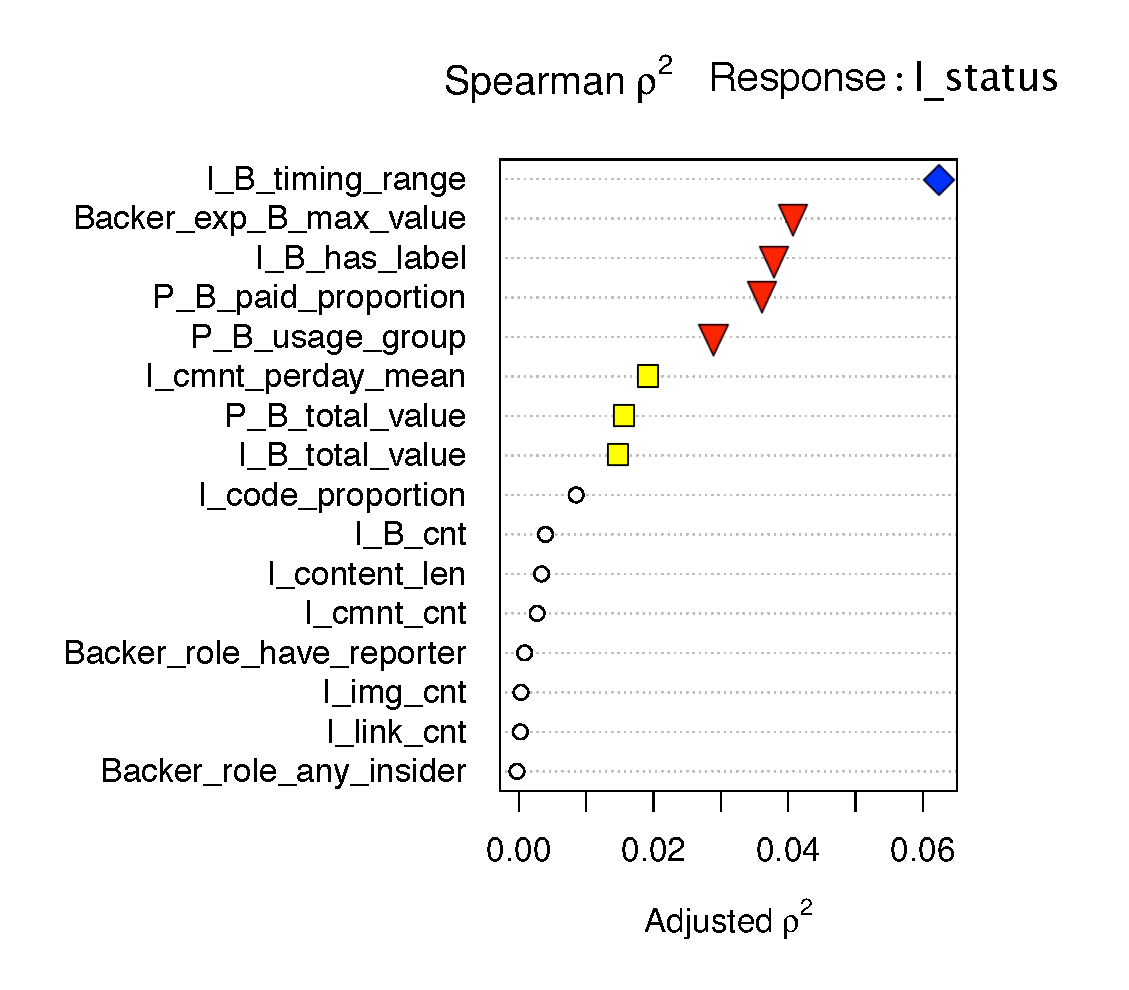
\includegraphics[width=\columnwidth]{pics/rq3/rq3_spearman}
        \caption{Dotplot of the Spearman multiple ${\rho}^2$  of each factor in all the bounty issue reports. The larger the ${\rho}^2$ value, the more likely the factor has a non-linear relationship with the response variable. By observing the rough clustering of the factors according to their $\rho^2$, we cluster the factors into four groups according
        to the Spearman multiple $\rho^2$  values. We assign the first, second, and third groups of factors (categorized by the ${\rho}^2$ value) which are highlighted with a blue diamond, red triangle, and yellow square, 5, 4, and 3 degrees of freedom, respectively.  }
        \label{fig:rq3_spearman}
      \end{figure}

    \item \textbf{Non-linear Term Allocation:}
      Similar to prior work~\cite{mcintosh2016empirical, wang2017understanding}, we add non-linear terms (i.e., NL) in each model to capture the more complex relationship in the data by employing restricted cubic splines~\cite{Harrell:2006}. The non-linear factor will be assigned more degrees of freedom (i.e., D.F.). We calculated the Spearman multiple $\rho^2$ between the dependent factor and each explanatory factor to measure their non-linear relationship. If a factor has a higher $\rho^2$, it indicates that it has a higher chance of having a non-linear relationship with the dependent factor. We therefore assigned this factor more degrees of freedom.
      Figure~\ref{fig:rq3_spearman} shows the Spearman multiple $\rho^2$ of the studied factors. By observing the rough clustering of the
      factors according to their $\rho^2$, we cluster the factors into four groups according to the Spearman multiple $\rho^2$  values. The factor marked by the blue diamond is assigned five degrees, factors marked by red triangles are assigned four degrees and factors marked by yellow squares are assigned three degrees of freedom.
      We use the R package \textbf{rms}\footnote{\url{https://cran.r-project.org/web/packages/rms/index.html}} to implement our logistic regression model.

      \item \textbf{Logistic Regression Model Building:} Finally, we built four groups of logistic regression models (i.e., the first-timer, moderate, frequent, and global models) based on 100 samples and ended up with 400 models.


	\end{enumerate}
	
	
	
%=================== Model analysis =================%

      \section{Model analysis}
      In this section, we elaborate on the details of our model analysis process. The process includes two parts:
      \begin{enumerate}
      	\item \textbf{Model Assessment:}  For a logistic regression model, we use the Area Under the Receiver Operating Characteristic Curve (i.e., AUC) and a bootstrap-derived approach \cite{efron1986biased} to assess the explanatory power of the models following prior studies~\cite{mcintosh2016empirical,wang2017understanding,kabinna2018examining}. The AUC ranges from 0 to 1 (0.5 is the performance of a random guessing model) and a higher AUC means that the model has a higher ability to capture the relationships between the explanatory factors and the response factor.

     		 For each sample, we use a bootstrap-derived approach~\cite{efron1986biased} to validate the performance of models. We first build a model with a bootstrapped sample and calculate the AUC (i.e., the \textit{bootstrapped\_AUC}). Then we apply the model to the original sample and calculate the AUC (i.e., the \textit{original\_AUC}). After that, we use the optimism value, which is the difference between the \textit{bootstrapped\_AUC} and \textit{original\_AUC} to evaluate the degree of overfitting of the model. A small optimism value indicates that the model does not suffer from overfitting.
    		  We repeated the bootstrap-derived approach for 100 iterations for each sample and used the median \textit{bootstrapped\_AUC} and the median optimism value to represent the performance of models for that sample.
    		  Finally, we built 10,000 (100 samples * 100 bootstrap-derived iterations) models for each group of models.
     		 For each group of models, we use the median optimism value and the median AUC of all samples to evaluate the stability of the models. In order to condense our writing, we use the \textit{median AUC} and the \textit{median optimism value} to express the above concepts.
     		 
         \item \textbf{Explanatory Variables Analysis:}   
			We further study the impact of each factor on the issue-addressing likelihood by using the \textbf{anova} function in the R \textbf{rms} package to compute the Wald $\chi^2$ value.
  		    The larger the Wald $\chi^2$ value of a factor is, the larger impact of the factor on the issue-addressing likelihood.
   			For each sample, we computed the Wald $\chi^2$ value for each factor. Then we use the median Wald $\chi^2$ value of each factor to represent the impact of that factor.

    		In addition, to further understand how a factor influences the value of the response variables, we use the \textbf{Predict} function in the \textbf{rms} R package to plot the estimated issue-addressing likelihood against a factor. %Since all models across 100 samples showed similar patterns of influence for the factors, we randomly selected a sample as an example to build models and visualize the results (see Figure~\ref{fig:rq3_trend}).
      		%The analysis allows us to further understand how a factor affects the issue-addressing likelihood. %We hold the other factors at their median values when exploring a specific factor.
      \end{enumerate}
      Table~\ref{tab:rq3_analysis} shows the results of our model analysis. 

   
       % Table generated by Excel2LaTeX from sheet 'Sheet2'
       \begin{table*}[]
      % \tiny
         \centering
         \caption{The results of the model analysis for four groups of models. We highlight the most important variable of models of each group in bold. The \textbf{NL} indicates the non-linear term and the \textbf{D.F.} indicates the degree of freedom.}
           \begin{tabular}{lp{0.5cm}p{0.8cm}rp{0.9cm}rp{0.8cm}rp{0.8cm}r}
           \toprule
           \multicolumn{2}{p{1.7cm}}{} & \multicolumn{2}{p{8em}}{\textbf{Global Models}} & \multicolumn{2}{p{1.7cm}}{\textbf{First-timer Model}s} & \multicolumn{2}{p{1.7cm}}{\textbf{Moderate Models}} & \multicolumn{2}{p{1.7cm}}{\textbf{Frequent Models}} \bigstrut[b]\\
           \midrule
           \multicolumn{2}{p{8em}}{Median AUC} & \multicolumn{2}{l}{0.72} & \multicolumn{2}{l}{0.74} & \multicolumn{2}{l}{0.71} & \multicolumn{2}{l}{0.81} \bigstrut[t]\\
           \multicolumn{2}{p{15em}}{Median Optimism Value} & \multicolumn{2}{l}{0.02} & \multicolumn{2}{l}{0.03} & \multicolumn{2}{l}{0.04} & \multicolumn{2}{l}{0.03} \bigstrut[b]\\
           \midrule
           \multicolumn{2}{l}{Factors} & Overall & \multicolumn{1}{p{3em}}{NL} & Overall & \multicolumn{1}{p{3em}}{NL} & Overall & \multicolumn{1}{p{3em}}{NL} & Overall & \multicolumn{1}{p{3em}}{NL} \bigstrut\\
           \midrule
           \multicolumn{1}{l}{\multirow{2}[2]{*}{I\_B\_timing\_range}} & D.F.  & 1     &       & 1     &       & 1     &       & 1     &  \bigstrut[t]\\
                 & $\chi^2$ & \textbf{47.87***} &       &6.68* &       & \textbf{18.12***} &       & \textbf{21.26***} &  \bigstrut[b]\\
           \midrule
           \multicolumn{1}{l}{\multirow{2}[2]{*}{P\_B\_usage\_group}} & D.F.  & 1     &       & -     &       & -     &       & -     &  \bigstrut[t]\\
                 & $\chi^2$ & \textbf{28.38***} &       & -     &       & -     &       & -     &  \bigstrut[b]\\
           \midrule
           \multicolumn{1}{l}{\multirow{2}[2]{*}{I\_B\_total\_value}} & D.F.  & 2     & \multicolumn{1}{p{4em}}{1} & 2     & \multicolumn{1}{p{3em}}{1} & 2     & \multicolumn{1}{p{3em}}{1} & 2     & \multicolumn{1}{p{5.085em}}{1} \bigstrut[t]\\
                 & $\chi^2$ & 9.58** & \multicolumn{1}{p{4em}}{7.21**} & \textbf{23.06***} & \multicolumn{1}{p{3em}}{0.13} & 2.0   & \multicolumn{1}{p{3em}}{0.31} & 6.57* & \multicolumn{1}{p{5.085em}}{4.81*} \bigstrut[b]\\
           \midrule
           \multicolumn{1}{l}{\multirow{2}[2]{*}{I\_code\_proportion}} & D.F.  & 1     &       & 1     &       & 1     &       & 1     &  \bigstrut[t]\\
                 & $\chi^2$ & 10.97** &       & 1.97  &       & 6.20* &       & 1.96  &  \bigstrut[b]\\
           \midrule
           \multicolumn{1}{l}{\multirow{2}[2]{*}{I\_B\_has\_label}} & D.F.  & 1     &       & 1     &       & 1     &       & 1     &  \bigstrut[t]\\
                 & $\chi^2$ & 14.75*** &       & 4.40* &       & 3.41  &       & 0.93  &  \bigstrut[b]\\
           \midrule
           \multicolumn{1}{l}{\multirow{2}[2]{*}{Backer\_exp\_B\_max\_value}} & D.F.  & 3     & \multicolumn{1}{p{4em}}{2} & 3     & \multicolumn{1}{p{3em}}{2} & 3     & \multicolumn{1}{p{3em}}{2} & 3     & \multicolumn{1}{p{5.085em}}{2} \bigstrut[t]\\
                 & $\chi^2$ & 9.14* & \multicolumn{1}{p{4em}}{7.88*} & 1.39  & \multicolumn{1}{p{3em}}{0.23} & 2.13  & \multicolumn{1}{p{3em}}{0.67} & 13.55** & \multicolumn{1}{p{5.085em}}{12.87**} \bigstrut[b]\\
           \midrule
           \multicolumn{1}{l}{\multirow{2}[2]{*}{P\_B\_paid\_proportion}} & D.F.  & 3     & \multicolumn{1}{p{4em}}{2} & -     &       & 3     & \multicolumn{1}{p{3em}}{2} & 3     & \multicolumn{1}{p{5.085em}}{2} \bigstrut[t]\\
                 & $\chi^2$ & 11.22* & \multicolumn{1}{p{4em}}{4.98} & -     &       & 4.23  & \multicolumn{1}{p{3em}}{0.58} & 16.43** & \multicolumn{1}{p{5.085em}}{15.37***} \bigstrut[b]\\
           \midrule
           \multicolumn{1}{l}{\multirow{2}[2]{*}{P\_B\_total\_value}} & D.F.  & 2     & \multicolumn{1}{p{4em}}{1} & -     &       & 2     & \multicolumn{1}{p{3em}}{1} & 2     & \multicolumn{1}{p{5.085em}}{1} \bigstrut[t]\\
                 & $\chi^2$ & 9.85** & \multicolumn{1}{p{4em}}{8.96**} & -     &       & 1.40  & \multicolumn{1}{p{3em}}{0.10} & 15.42*** & \multicolumn{1}{p{5.085em}}{13.46***} \bigstrut[b]\\
           \midrule
           \multicolumn{1}{l}{\multirow{2}[2]{*}{I\_img\_cnt}} & D.F.  & 1     &       & 1     &       & 1     &       & 1     &  \bigstrut[t]\\
                 & $\chi^2$ & 1.62  &       & 1.25  &       & 0.79  &       & 1.28  &  \bigstrut[b]\\
           \midrule
           \multicolumn{1}{l}{\multirow{2}[2]{*}{I\_link\_cnt}} & D.F.  & 1     &       & 1     &       & 1     &       & 1     &  \bigstrut[t]\\
                 & $\chi^2$ & 0.41  &       & 0.48  &       & 0.55  &       & 0.91  &  \bigstrut[b]\\
           \midrule
           \multicolumn{1}{l}{\multirow{2}[2]{*}{I\_content\_len}} & D.F.  & 1     &       & 1     &       & 1     &       & 1     &  \bigstrut[t]\\
                 & $\chi^2$ & 1.76  &       & 0.29  &       & 0.84  &       & 1.97  &  \bigstrut[b]\\
           \midrule
           \multicolumn{1}{l}{\multirow{2}[2]{*}{I\_cmnt\_perday\_mean}} & D.F.  & 2     & \multicolumn{1}{p{4em}}{1} & 2     & \multicolumn{1}{p{3em}}{1} & 2     & \multicolumn{1}{p{3em}}{1} & 2     & \multicolumn{1}{p{5.085em}}{} \bigstrut[t]\\
                 & $\chi^2$ & 7.60* & \multicolumn{1}{p{4em}}{2.52} & 4.42  & \multicolumn{1}{p{3em}}{0.15} & 1.32  & \multicolumn{1}{p{3em}}{0.58} & 1.28  & \multicolumn{1}{p{5.085em}}{} \bigstrut[b]\\
           \midrule
           \multicolumn{1}{l}{\multirow{2}[2]{*}{I\_B\_cnt}} & D.F.  & 1     &       & 1     &       & 1     &       & 1     &  \bigstrut[t]\\
                 & $\chi^2$ & 0.80  &       & 0.94  &       & 1.12  &       & 7.76** &  \bigstrut[b]\\
           \midrule
           \multicolumn{1}{l}{\multirow{2}[2]{*}{I\_cmnt\_cnt}} & D.F.  & 1     &       & 1     &       & 1     &       & 1     &  \bigstrut[t]\\
                 & $\chi^2$ & 0.35  &       & 1.72  &       & 0.30  &       & 2.10  &  \bigstrut[b]\\
           \midrule
           \multicolumn{1}{l}{\multirow{2}[2]{*}{Backer\_role\_any\_insider}} & D.F.  & 1     &       & 1     &       & 1     &       & 1     &  \bigstrut[t]\\
                 & $\chi^2$ & 1.78  &       & 5.81* &       & 0.32  &       & 0.67  &  \bigstrut[b]\\
           \midrule
           \multicolumn{1}{l}{\multirow{2}[1]{*}{Backer\_role\_have\_reporter}} & D.F.  & 1     &       & 1     &       & 1     &       & 1     &  \bigstrut[t]\\
                 & $\chi^2$ & 0.52  &       & 0.45  &       & 0.69  &       & 0.38  &  \\
                 \bottomrule
      \multicolumn{10}{l}{P-value of the $\chi^2$ test: `***' $<$ 0.001; `**' $<$ 0.01; `*' $<$ 0.05} \bigstrut[t]\\
           \end{tabular}%
         \label{tab:rq3_analysis}%
       \end{table*}%


      \section{Additional result for threats to validity}

      \begin{figure*}[th]
        \centering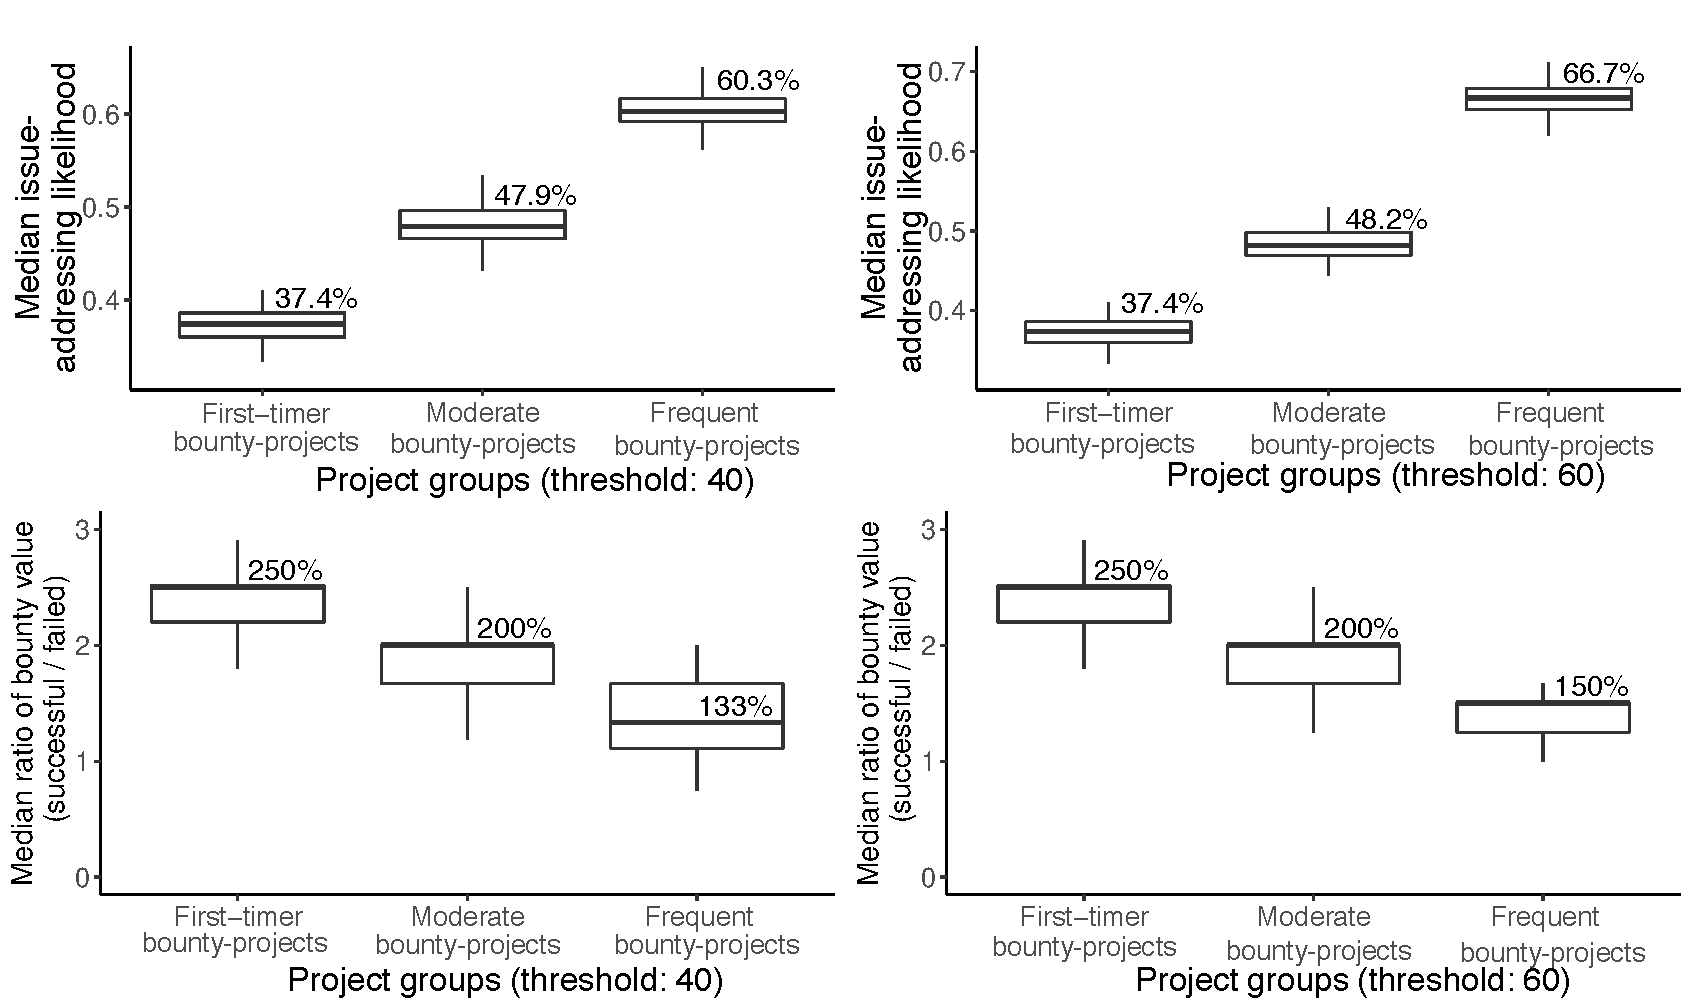
\includegraphics[width=\textwidth ]{pics/threat/threat}
        \caption{The distribution of the median issue-addressing likelihood and the median ratio of bounty value when using different thresholds for the separation across different project groups.}
        \label{fig:threat}
      \end{figure*}
      In this section, we visualize the result of our analysis in the threats to validity section regarding different bounty-usage frequency thresholds. Figure~\ref{fig:threat} shows  the distribution of the median issue-addressing likelihood and the median ratio of bounty value when using different thresholds for the separation across different project groups. Figure~\ref{fig:threat} shows that our results are not affected by our choice for the threshold for the bounty-usage frequency.

      \balance
      \bibliographystyle{abbrv}
      {
      \footnotesize
      \bibliography{ref}
      }
  \end{appendices}
\end{document}
